%&<latex>
\documentclass[11pt]{exam}
\pagestyle{plain}
\usepackage{anysize}
\papersize{11in}{8.5in}
\marginsize{1in}{1in}{.5in}{.5in}
\pagenumbering{arabic}
\usepackage{setspace}
\usepackage[usenames]{color}
\usepackage[fleqn]{amsmath}
\usepackage{amssymb}
\usepackage{graphicx}
\usepackage{indentfirst}
\usepackage{ragged2e}
\usepackage{upgreek}
\usepackage{xspace}
\usepackage{ifthen}
\usepackage{parskip}
\usepackage[normalem]{ulem}
\usepackage[round]{natbib}
\bibliographystyle{evolution}
\usepackage{hyperref}
\hypersetup{pdfborder={0 0 0}, colorlinks=true, urlcolor=blue, linkcolor=blue, citecolor=blue}
\usepackage{enumitem}
\usepackage{tabularx}
\usepackage{wrapfig}
\usepackage{tikz}
\usetikzlibrary{arrows}

\newcolumntype{L}{>{\raggedright\arraybackslash}X}%
\newcolumntype{R}{>{\raggedleft\arraybackslash}X}%
\newcolumntype{C}{>{\centering\arraybackslash}X}%

\newcommand{\myIfArg}[2]{\ifthenelse{\equal{#1}{}}{}{#2}}

\providecommand{\e}[1]{\ensuremath{\times 10^{#1}}}
\newcommand{\ifTwoArgs}[3]{\ifthenelse{\equal{#1}{}\or\equal{#2}{}}{}{#3}\xspace}
\newcommand{\ifArg}[2]{\ifthenelse{\equal{#1}{}}{}{#2}\xspace}

\makeatletter
\newcommand*{\rom}[1]{\expandafter\@slowromancap\romannumeral #1@}
\makeatother

%% Basic formatting and spacing %%%%%%%%%%%%%%%%%%%%%
% \setlength{\parindent}{0em}
% \setlength{\parskip}{0.5em}

\tikzstyle{centered} = [align=center, text centered, font=\sffamily\bfseries]
\tikzstyle{skip} = [centered, inner sep=0pt, fill]
\tikzstyle{empty} = [centered, inner sep=0pt]
\tikzstyle{inode} = [centered, circle, minimum width=4pt, fill=black, inner sep=0pt]
\tikzstyle{tnode} = [centered, circle, inner sep=1pt]

\begin{document}
% \printanswers

\begin{table}
\begin{tabular*}{\textwidth}{@{\extracolsep{\fill}} l l l }
    \textbf{\large Analyzing Natural Selection} & BIOL 180 & September 30 2014 \\
\end{tabular*}
\end{table}

\begin{table}
    \small
\begin{tabularx}{\textwidth}{ L L L }
    Name \hrulefill & Name \hrulefill & Name \hrulefill \\
\end{tabularx}
\end{table}


\begin{wrapfigure}{r}{0.3\textwidth}
  \vspace{-0.5em}
  \begin{center}
    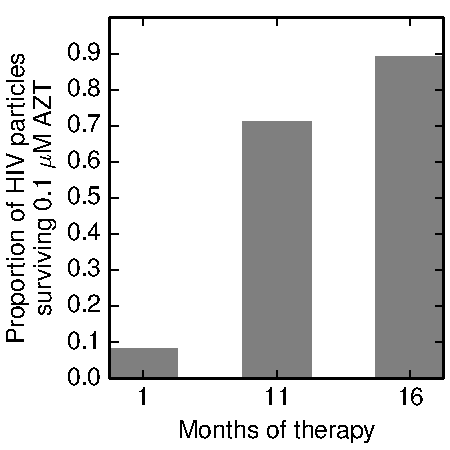
\includegraphics[width=0.3\textwidth]{../../images/hiv-survival-plot.pdf}
  \end{center}
  \vspace{-1.5em}
\end{wrapfigure}

Infection with the human immunodeficiency virus (HIV) causes the fatal disease
called AIDS. The first drug that was effective against HIV was AZT. When AZT
was first administered to HIV-infected patients, virus populations dropped
dramatically. But with time, HIV populations in the treated patients rebounded
and the patients died of AIDS. (Note: inside an infected person, individual HIV
particles live for about a day, on average.)

% \begin{figure}[htbp]
%     \centering
%     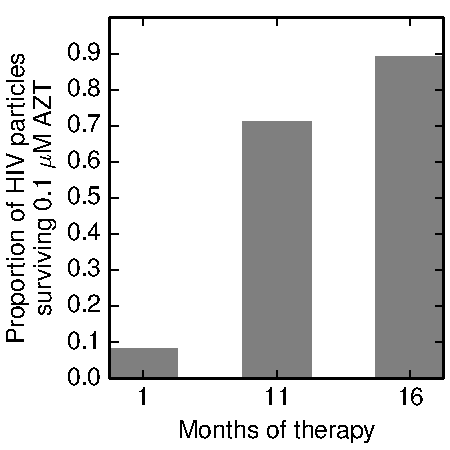
\includegraphics[width=0.3\textwidth]{../../images/hiv-survival-plot.pdf}
%     \label{figSurvival}
% \end{figure}

The data graphed to the right are from virus particles that were isolated from
a patient at different times after AZT therapy began.
After being isolated from the patient, the virus particles were exposed to 0.1
$\mu$M AZT.

% \vspace{1cm}

\begin{questions}

\question
The researchers who did the study claim that it supports the hypothesis that
the HIV population in this patient evolved resistance to AZT. Do you agree?
Defend your answer.

\begin{solution}
    Yes---over time, the proportion that survive in the presence of AZT
    increases. The data are consistent with the hypothesis that natural
    selection favored virus particles that can survive in the presence of AZT.
\end{solution}

\vspace*{\stretch{1}}

\question
AZT and other antiviral drugs work by binding to molecules that help HIV
produce offspring inside a host cell.  The binding is very specific---if the
shape or composition of the target molecule changes, the drug may not work.

AZT binds at a specific location on a molecule called reverse transcriptase.
HIV has a gene that contains the information for making reverse transcriptase.
But the genetic information varies among HIV particles. As a result, the
structure and composition of reverse transcriptase varies among HIV particles.

Based on this information, is there \textbf{heritable variation} in the
``resistance to AZT'' trait? Explain why or why not.

\begin{solution}
    Yes---because not all genes and versions of reverse transcriptase are
    alike, there is variation. And because AZT resistance depends on the
    structure of reverse transcriptase, and because the genetic information for
    making reverse transcriptase is passed on to offspring, the trait is
    heritable.
\end{solution}

\vspace*{\stretch{1}}

\question
Using the information in question 2 and the data in the graph, is it reasonable
to infer that there is \textbf{differential reproductive success} among HIV
with respect to the ``resistance to AZT'' trait? Explain why or why not.

\begin{solution}
    Yes---HIV particles that have AZT-resistant forms of reverse transcriptase
    should should have greater survival and reproduction in the presence of AZT
    than particles with non-resistant forms of reverse transcriptase.
\end{solution}

\vspace*{\stretch{1}}

\question
Did forms of reverse transcriptase that were resistant to AZT exist in the HIV
population before the patient began receiving AZT? Explain why or why not.

\begin{solution}
    Yes---among all the types of reverse transcriptase present in the
    population, it is almost certain that by chance some were at least slightly
    resistant to AZT.
\end{solution}

\vspace*{\stretch{1}}
\newpage

\question
When AZT is administered to a particular patient, does each individual HIV
particle inside that patient change to become more resistant to the drug, so
that eventually the HIV population would consist of drug-resistant forms?
Defend your answer.

\begin{solution}
    No---the HIV particles themselves do not change. The resistant individuals
    simply survive better and leave more offspring than the individuals that
    have less or no resistance to AZT.
\end{solution}

\vspace*{\stretch{1}}

\question
Physicians now have many drugs that they can prescribe for HIV-infected
individuals, in addition to AZT. So if HIV populations begin rebounding in a
patient who is receiving AZT, the patient stops taking AZT and switches to
different drugs. When the environment inside the patient changes in this way,
HIV populations again drop dramatically. Explain why.

\begin{solution}
    Initially, very few HIV particles in the population have resistance to the
    new drugs---most are susceptible and produce very few or no offspring.
\end{solution}

\vspace*{\stretch{1}}

\question
When a patient stops taking AZT and switches to new drugs, predict whether
AZT-resistant forms become more common, less common, or remain at the same
frequency, in that patient. Explain your logic.

\begin{solution}
    The AZT-resistant forms should become much less common, as that trait is no
    longer advantageous in the new environment. Forms that are resistant to the
    new drugs should become more common.
\end{solution}

\vspace*{\stretch{1}}

\question
Suppose the patient stopped taking AZT after several months and switched to a
new drug called a protease inhibitor (PI). On the axes below, use a solid line
to predict how the frequency of AZT-resistant forms will change over time. Use
a dotted line to predict how the frequency of PI-resistant forms will change
over time, and a dotted line to predict the frequency of HIV particles that are
resistant to both drugs.

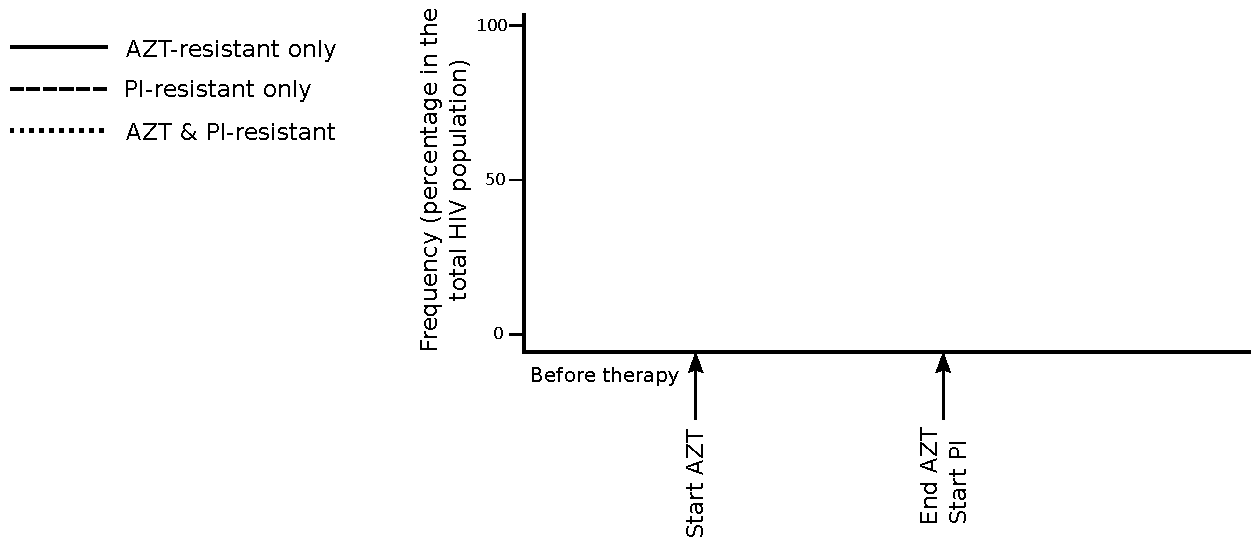
\includegraphics[width=0.9\textwidth]{../../images/hiv-frequency-plot.pdf}

\begin{solution}
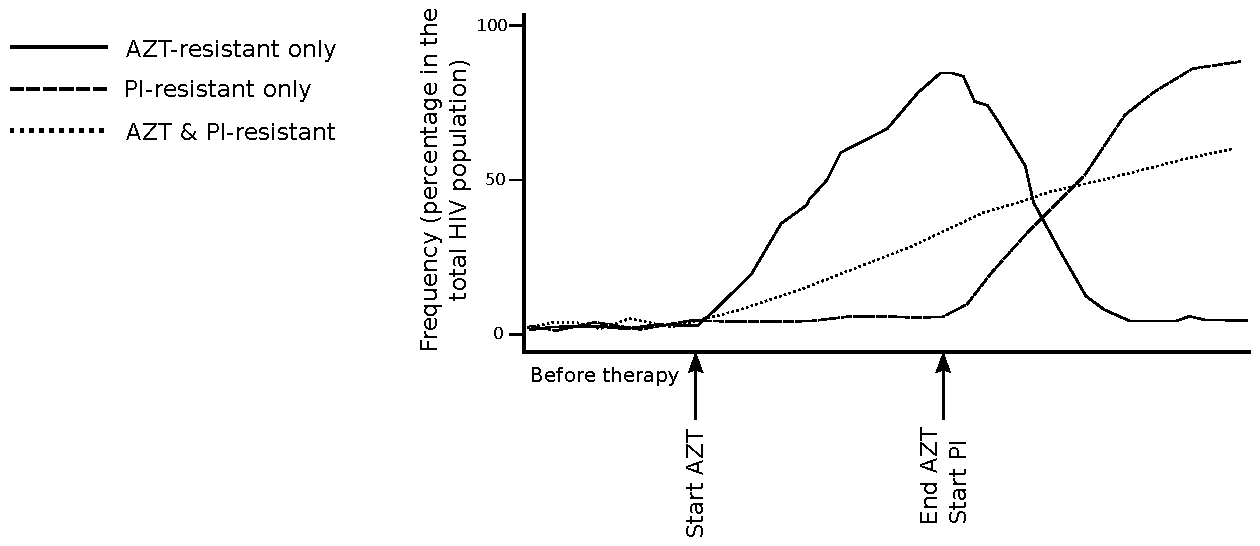
\includegraphics[width=0.9\textwidth]{../../images/hiv-frequency-plot-key.pdf}
\end{solution}

\end{questions}

\begin{center}
    \fbox{\parbox{\textwidth}{\centering
        Please turn the completed exercise in to your T.A. (and make sure that
        your names are legible!)
        }}
\end{center}


If you finish early, consider the following: Some humans have genes that either
(a) reduce the likelihood of HIV infection or (b) delay the onset of AIDS if an
infection does occur.

\begin{itemize}
    \item In human populations where HIV infection is common, are the
        frequencies of these ``resistance genes'' increasing, decreasing, or
        staying about the same? Explain your reasoning.

        \vspace{0.5cm}

    \item In human populations where HIV infection is rare, are the frequencies
        of these resistance genes increasing, decreasing, or staying about the
        same? Explain your reasoning.
\end{itemize}

\end{document}
